%%% ======= Beamer ======
\documentclass[usenames,dvipsnames,t]{beamer}
% \documentclass[usenames,dvipsnames, handout]{beamer}
\beamertemplatenavigationsymbolsempty % remove toolbar at the bottom of slides
\usepackage{appendixnumberbeamer} % for appendix
\usetheme{Madrid}
\usecolortheme{default}
\useinnertheme{circles}

\usepackage{fontawesome}

% Define commands for social media icons with links
\newcommand{\twitter}{\href{https://twitter.com/ThibeauWouters}{\textcolor{black}{\faTwitter}}}
\newcommand{\linkedin}{\href{https://www.linkedin.com/in/ThibeauWouters}{\textcolor{black}{\faLinkedin}}}
\newcommand{\github}{\href{https://github.com/ThibeauWouters}{\textcolor{black}{\faGithub}}}

\newcommand{\thetaeos}{\boldsymbol{\theta}_{\rm{EOS}}}
\newcommand{\boldtheta}{\boldsymbol{\theta}}

\setbeamercolor{author in head/foot}{bg=blue!10, fg=blue}
\setbeamercolor{title in head/foot}{bg=blue!10, fg=blue}
\setbeamercolor{date in head/foot}{bg=blue!10, fg=blue}

\makeatletter
\setbeamertemplate{footline}{
  \leavevmode%
  \hbox{%
  \begin{beamercolorbox}[wd=.333333\paperwidth,ht=2.25ex,dp=1ex,center]{author in head/foot}%
    \usebeamerfont{author in head/foot}\insertshortauthor\expandafter\ifblank\expandafter{\beamer@shortinstitute}{}{~~(\insertshortinstitute)}
  \end{beamercolorbox}%
  \begin{beamercolorbox}[wd=.333333\paperwidth,ht=2.25ex,dp=1ex,center]{title in head/foot}%
    \usebeamerfont{title in head/foot}\insertshorttitle
  \end{beamercolorbox}%
  \begin{beamercolorbox}[wd=.333333\paperwidth,ht=2.25ex,dp=1ex,right]{date in head/foot}%
    \usebeamerfont{date in head/foot}\insertshortdate{}\hspace*{2em}
    \insertframenumber{}%
%     / \inserttotalframenumber
    \hspace*{2ex} 
  \end{beamercolorbox}}%
  \vskip0pt%
}
\makeatother

\colorlet{beamer@blendedblue}{blue!70} % change color theme

\usepackage[style=numeric-comp,sorting=none,backend=biber]{biblatex}%<- specify style
\addbibresource{references.bib}%<- specify bib file

\usepackage{svg}


% For appendix
\newcommand{\backupbegin}{
   \newcounter{framenumberappendix}
   \setcounter{framenumberappendix}{\value{framenumber}}
}
\newcommand{\backupend}{
   \addtocounter{framenumberappendix}{-\value{framenumber}}
   \addtocounter{framenumber}{\value{framenumberappendix}} 
}

\setbeamertemplate{bibliography item}{\insertbiblabel} % improved references



% Other preamble stuff:
\usepackage{preamble}

%%% Uncomment for another color palette
% \definecolor{Logo1}{rgb}{0.0, 0, 0.7}
% \definecolor{Logo2}{rgb}{2.55, 2.55, 2.55}

% \setbeamercolor*{palette primary}{bg=Logo1, fg=white}
% \setbeamercolor*{palette secondary}{bg=Logo2, fg=white}
% \setbeamercolor*{palette tertiary}{bg=white, fg=Logo1}
% \setbeamercolor*{palette quaternary}{bg=white,fg=white}
% \setbeamercolor{structure}{fg=Logo1} % itemize, enumerate, etc
% \setbeamercolor{section in toc}{fg=Logo1} % TOC sections

% For figures
\usepackage{import}
\usepackage{xifthen}
\usepackage{pdfpages}
\usepackage{transparent}
\usepackage{mdframed}
\usepackage{subcaption}

\setbeamertemplate{caption}[numbered]



% --- Inkscape figures:
\newcommand{\incfig}[2][0.75\textwidth]{%
    \def\svgwidth{\columnwidth}
    \resizebox{#1}{!}{\import{Inkscape figs/}{#2.pdf_tex}}
}

% --- Height of frame
\newlength{\myheight}
\setlength{\myheight}{7cm}

\newlength\myheightfigureintext
\newlength\mydepthfigureintext
\settototalheight\myheightfigureintext{Xygp}
\settodepth\mydepthfigureintext{Xygp}
\setlength\fboxsep{0pt}


%------------------------------------------------------------
%This block of code defines the information to appear in the
%Title page
\title[\textsc{jester}] %optional
{Leveraging Differentiable Programming in the Inverse Problem of Neutron Stars}

\author[Thibeau Wouters]{\small{\textbf{Thibeau Wouters}, Peter T. H. Pang, Rahul Somasundaram, Ingo Tews, Tim Dietrich, and Chris Van Den Broeck} \\ \vspace{2mm} \href{mailto:t.r.i.wouters@uu.nl}{t.r.i.wouters@uu.nl} \newline \github \quad \linkedin \quad \twitter}


\date{Extreme Matter 17/03/2025}



%End of title page configuration block
%------------------------------------------------------------



%------------------------------------------------------------
%The next block of commands puts the table of contents at the 
%beginning of each section and highlights the current section:

%------------------------------------------------------------


\begin{document}

{

\usebackgroundtemplate{\transparent{0.15}{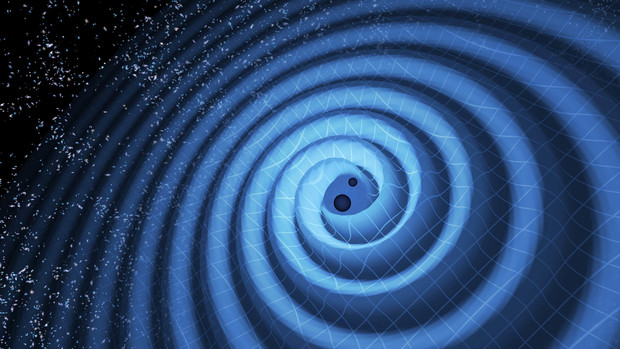
\includegraphics[width=\paperwidth,height=\paperheight]{Figures/GW-2.jpeg}}}

\begin{frame}[plain]
\titlepage

\begin{columns}
  \column{0.35\textwidth}
  \begin{figure}
    \centering
    \vspace{1.5mm}
    
\includegraphics[width=0.75\linewidth]{Figures/utrecht-university.png}
  \end{figure}
  \column{0.35\textwidth}
  \begin{figure}
    \centering
    
\includegraphics[width=0.75\linewidth]{Figures/Nikhef_logo-transparent.png}
  \end{figure}
\end{columns}


%%% as subfigures
% \begin{figure}
%   \centering
%   \begin{subfigure}[b]{0.475\textwidth}
%     \centering
%     
\includegraphics[width=0.6\textwidth]{Figures/utrecht-university.png}
%   \end{subfigure}
%   \caption*{}
%   \hfill
%   \begin{subfigure}[b]{0.475\textwidth}
%     \centering
%     
\includegraphics[width=0.6\textwidth]{Figures/Nikhef_logo-transparent.png}
%   \end{subfigure}
%   \caption*{}
%   % \caption*{}
% \end{figure}

\end{frame}
}

% %The next statement creates the title page.
% \frame[plain]{\titlepage



% }


%---------------------------------------------------------
%This block of code is for the table of contents after
%the title page
% \begin{frame}[plain, noframenumbering]
% \frametitle{Table of Contents}
% \tableofcontents
% \end{frame}
%---------------------------------------------------------


\begin{frame}{Introduction -- Motivation}
  \def\x{4mm}
  
  Neutron stars (NSs) offer unique probes of the high-density regime of the equation of state (EOS) of dense nuclear matter.

  \vspace{\x}

  \red{Inverse problem of NSs}: infer the EOS from observations of NSs (masses, radii, tidal deformabilities, \dots)

  \begin{figure}
    \centering
    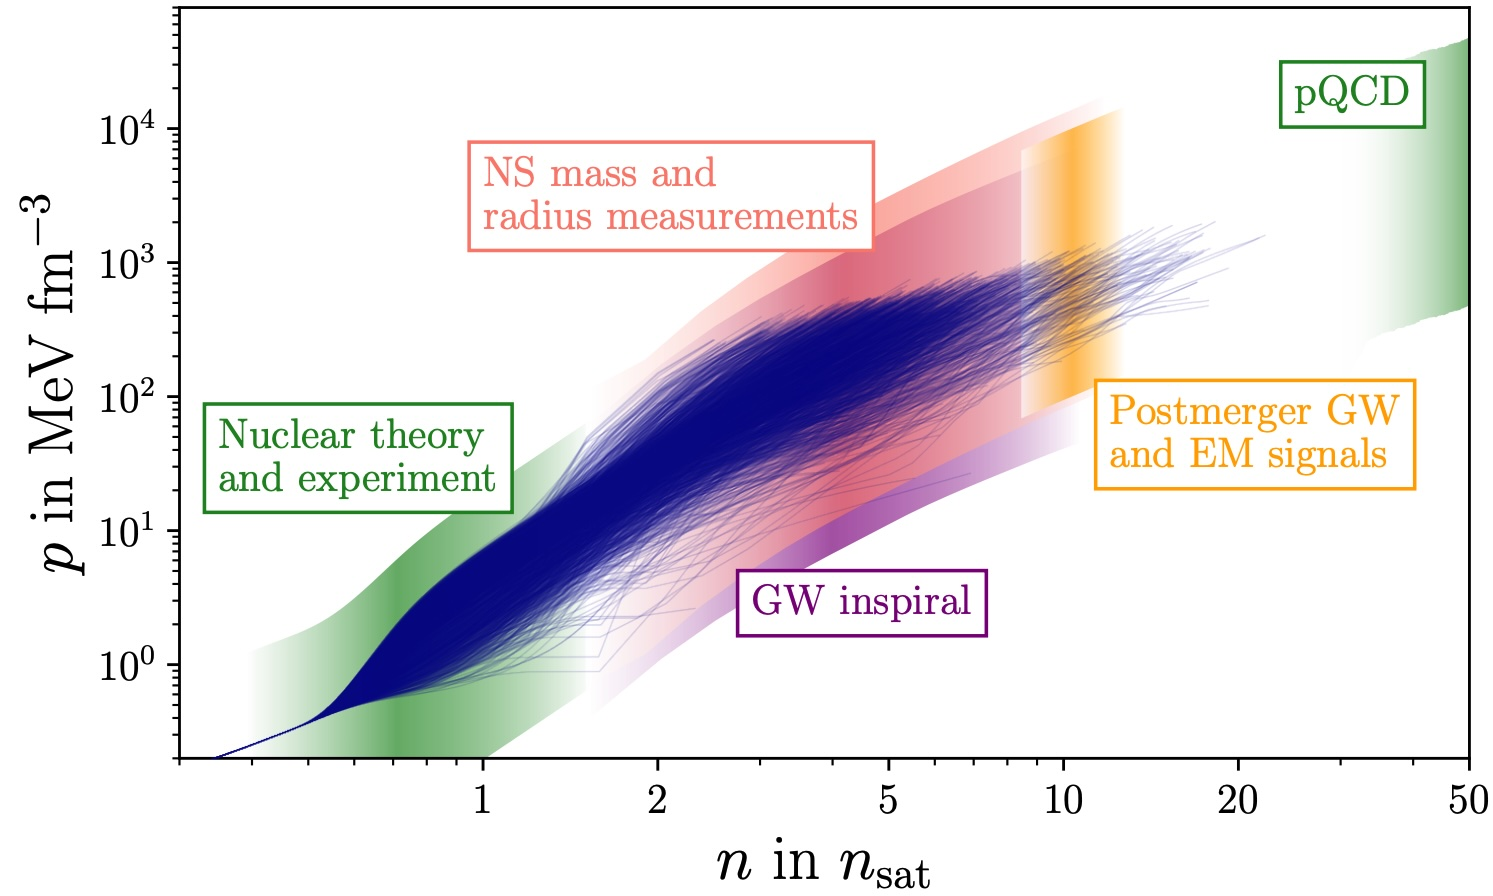
\includegraphics[width=0.75\linewidth]{Figures/Koehn_EOS.jpg}
  \end{figure}

\end{frame}

% \begin{frame}{Introduction -- Motivation}

%   \def\x{4mm}
  
%   \vspace{\x}

%   \begin{itemize}
%     \item Neutron stars (NSs) are unique probes of the equation of state (EOS) of dense nuclear matter ($\lesssim 8$ times the nuclear saturation density $n_{\rm{sat}} = 0.16 \ \rm{fm}^{-3}$)
    
%     \vspace{\x}

%     \item \red{Inverse problem of NSs}: infer EOS from observations of NSs (masses, radii, tidal deformabilities, \dots)
    
%     \vspace{\x}

%     \item Often solved with Bayesian inference: computationally expensive!

%   \end{itemize}

%   \vspace{\x}
  
%   \begin{tcolorbox}[colback=blue!10, boxrule=0pt]
%     \textbf{Challenge:} 3G GW detectors will observe $\mathcal{O}(10^5)$ BNS/year $\rightarrow$ need for efficient inference
%   \end{tcolorbox}
    
% \end{frame}

\begin{frame}{Introduction --  Differentiable programming with \textsc{jax}}
  \def\x{5mm}
  \def\y{7mm}

  Main bottleneck: solving Tolman-Oppenheimer-Volkoff equations

  \vspace{\x}
  
  Solution: \red{differentiable programming} with \textsc{jax}~\cite{frostig2018compiling}
  \begin{itemize}
    \vspace{\x}
    \item Automatic differentiation to compute gradients of functions
    
    \vspace{\x}
    
    \item Use efficient MCMC algorithm and GPU accelerators
  \end{itemize}

  \vspace{\x}

  Our contributions:

  \begin{itemize}
    \vspace{\x}

    \item Fast inference: $\sim 0.24$ ms per TOV call, $\sim 1$ h for full MCMC run

    \vspace{\x}

    \item \red{Novel tool} to study EOS: gradient descent on NS observables
  \end{itemize}

  \vspace{\y}
  
  Available open source: \textsc{jester} (\href{https://github.com/tsunhopang/jester}{{\faGithub \texttt{tsunhopang/jester}}})
\end{frame}


% \begin{frame}{Introduction --  Overview}
%   \def\x{2mm}

%   \begin{itemize}
%     \vspace{\x}
%     \item Bayesian inference
    
%     \begin{itemize}
%       \vspace{\x}
%       \item Equation of state parametrization and sampler
      
%       \vspace{\x}
      
%       \item Validation of methods and scaling
      
%       \vspace{\x}
      
%       \item Measuring breakdown of chiral effective field theory $\chi_{\rm{EFT}}$ from NSs
%     \end{itemize}

%     \vspace{\x}
%     \item Variational inference: gradient descent on NS observables
    
%   \end{itemize}

% \end{frame}


\begin{frame}{Methods -- Equation of state parametrization}

  \def\x{3mm}
  \def\y{3mm}

  % \begin{itemize}
  %   \vspace{\x}
    
  \red{Lower density} ($< 1-2 \ n_{\rm{sat}}$): metamodel~\cite{Margueron:2017eqc,Margueron:2017lup} 
  
  \begin{itemize}
    \vspace{\y}
    
    \item Taylor expansion of energy per nucleon $E/A$

    \vspace{\y}

    \item Nuclear empirical parameters ($E_{\rm{sym}}, L_{\rm{sym}}$, \dots, $E_{\rm{sat}}, K_{\rm{sat}}$, \dots)
  \end{itemize}

  \vspace{\x}

  \red{Higher density}: parametrize $c_s^2(n)$ with grid points and interpolation~\cite{Somasundaram:2021clp}

  \begin{figure}
    \centering
    \begin{subfigure}[b]{0.475\textwidth}
        \centering
        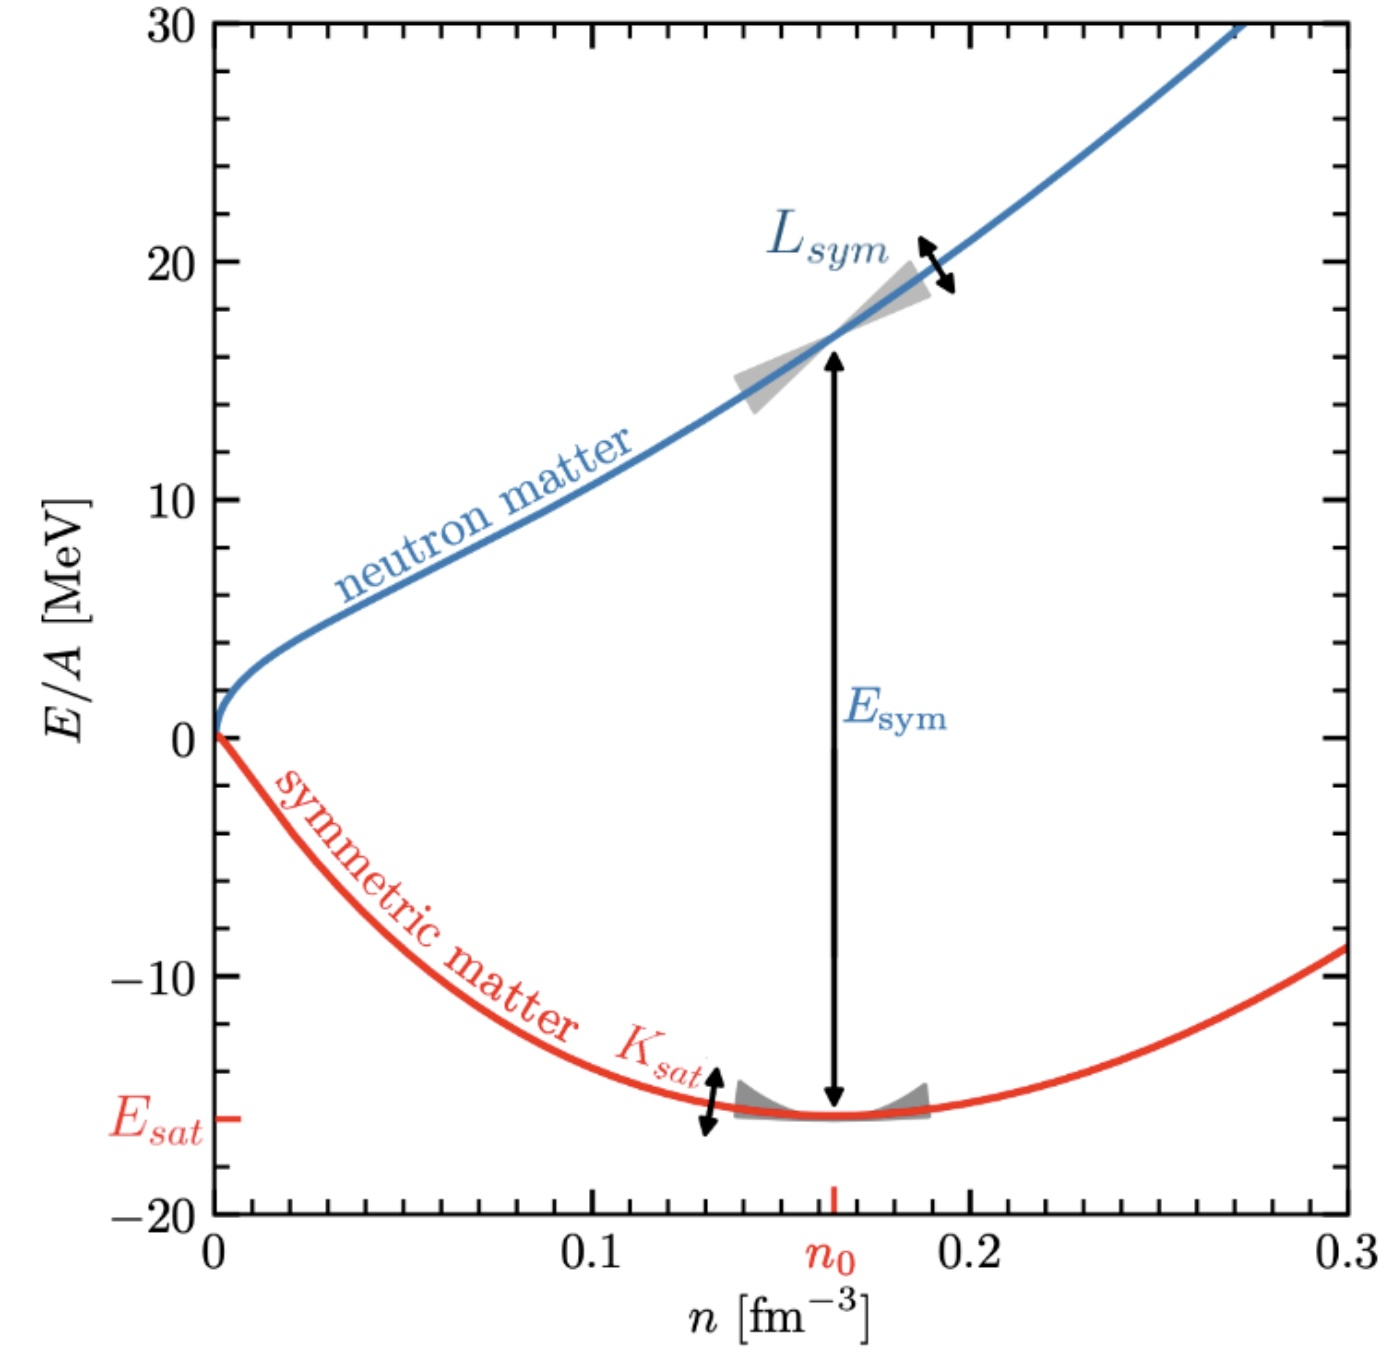
\includegraphics[width=0.75\textwidth]{Figures/metamodel_frank.jpg}
    \end{subfigure}
    \hfill
    \begin{subfigure}[b]{0.475\textwidth}
        \centering
        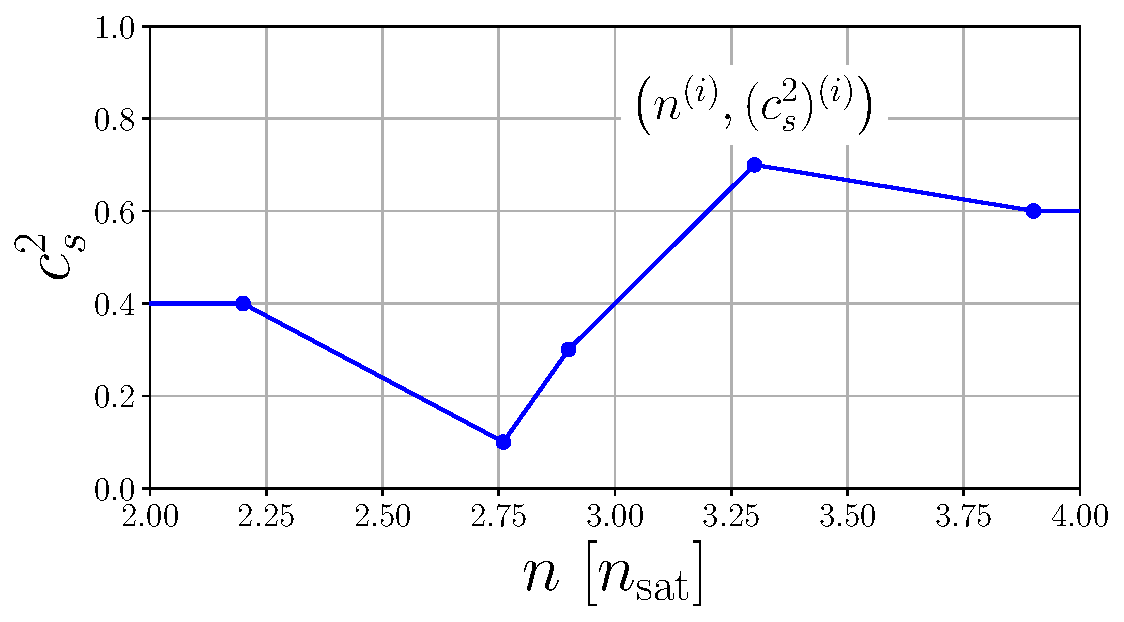
\includegraphics[width=0.75\textwidth]{Figures/cs2_sketch.pdf}
    \end{subfigure}
    % \caption{Three simple graphs}
    % \label{fig:three graphs}
\end{figure}


\end{frame}

\begin{frame}{Methods -- Bayesian inference}

  \def\x{6mm}
  \def\y{1mm}

  \red{Bayesian inference}: get \red{posterior} of EOS parameters $\theta_{\rm{EOS}}$ with Markov chain Monte Carlo (MCMC) and NS data $d$
  \begin{equation*}
      \red{p(\theta_{\rm{EOS}} | d)} \propto p(d | \theta_{\rm{EOS}}) p(\theta_{\rm{EOS}})
  \end{equation*}

  Computationally expensive: solve TOV equations for many $\theta_{\rm{EOS}}$!

  \begin{itemize}
    \vspace{\y}
    \item \texttt{JAX}: compile code, run on GPU
    
    \vspace{\y}
    \item \texttt{flowMC}~\cite{Gabrie:2021tlu,Wong:2022xvh}: MCMC with normalizing flows as proposal distributions
  \end{itemize}

  \vspace{\x}

  With this, we achieve (on NVIDIA H100 GPU)
  \begin{itemize}
    \vspace{\y}
    \item $\sim 0.24$ ms per TOV call
    
    \vspace{\y}
    \item Complete MCMC run in $\sim 1$ h 
  \end{itemize}
\end{frame}


\begin{frame}{Results -- Validation and scaling}

  \def\x{2mm}
  \def\y{2mm}

  \begin{itemize}
    \vspace{\y}
    \item EOS constraints: nuclear theory ($\chi_{\rm{EFT}}$), NS observations (heavy PSRs, NICER, GW170817)

    \vspace{\y}
    \item Extend Koehn+~\cite{Koehn:2024set} with complete EOS sampling

    \vspace{\y}
    \item Scales well with number of parameters (more $c_s^2(n)$ grid points)
  \end{itemize}

  \vspace{\x}

  \begin{columns}

    \column{0.5\textwidth}

    \begin{figure}[htpb]
      \centering
      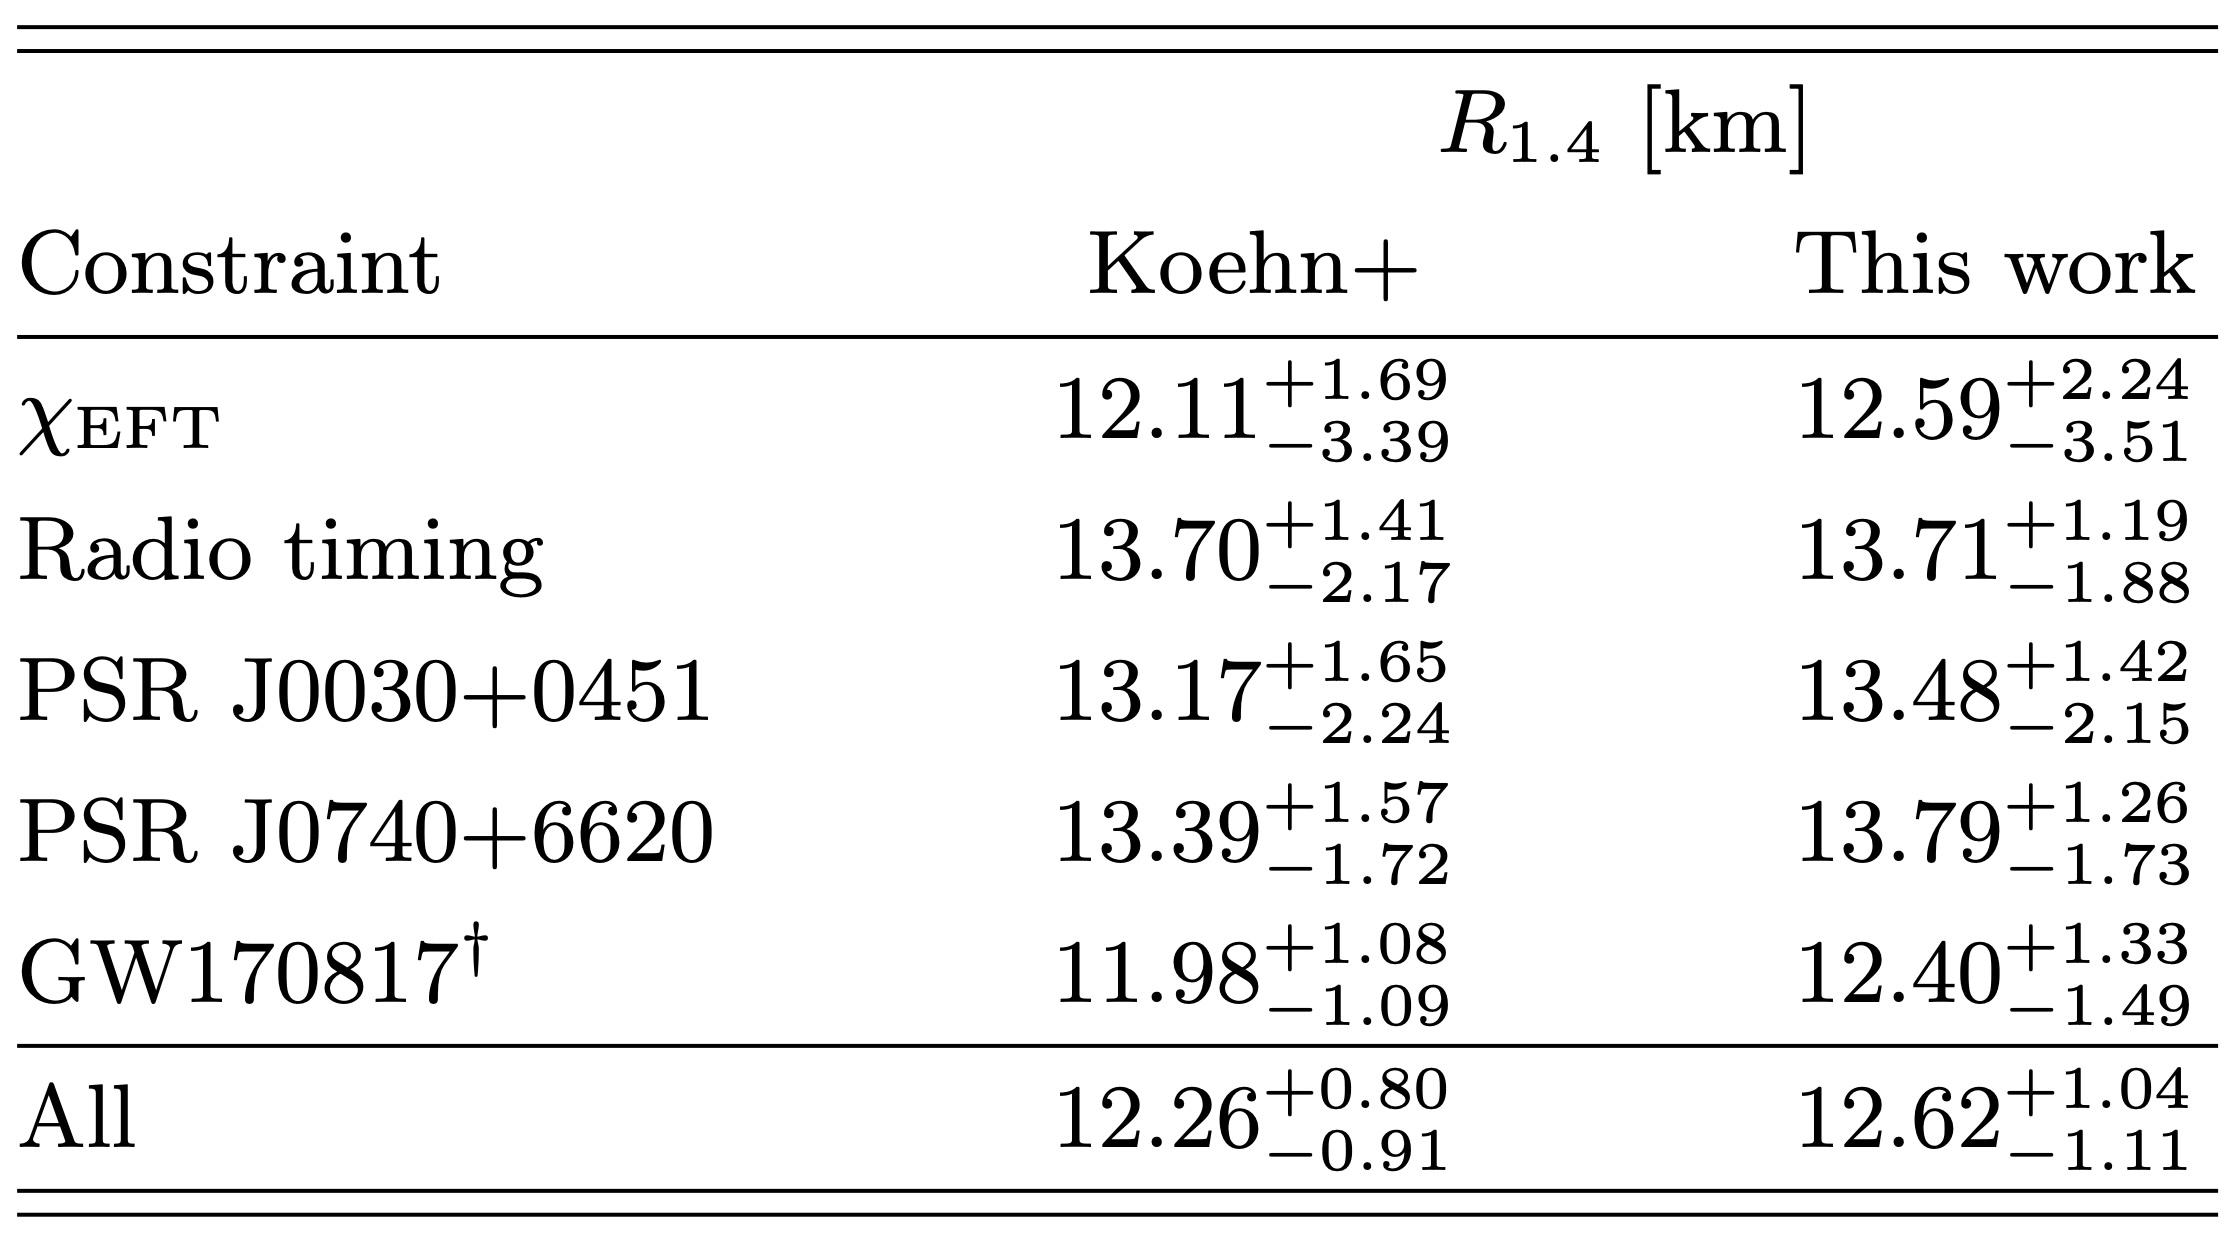
\includegraphics[width=0.975\linewidth]{Figures/R14_table.jpg}
    \end{figure}

    \column{0.5\textwidth}
    \begin{figure}[htpb]
      \centering
      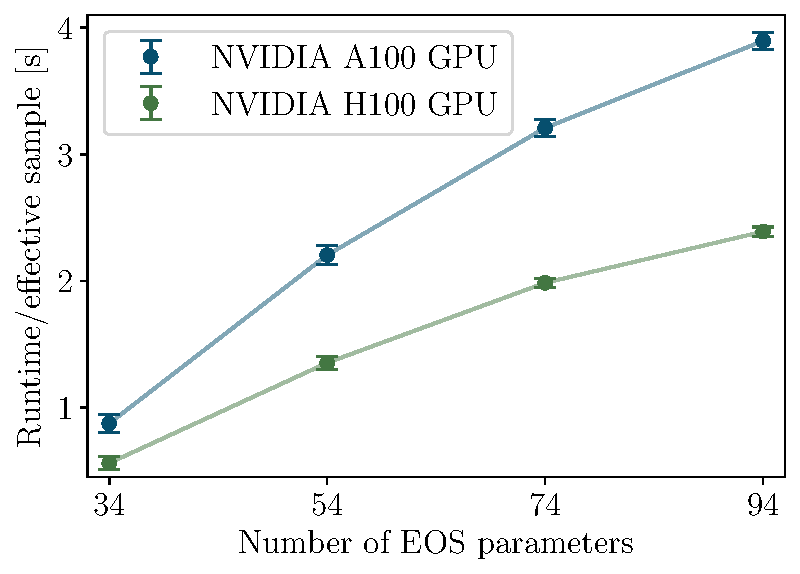
\includegraphics[width=0.975\linewidth]{Figures/scaling_plot.pdf}
    \end{figure}

  \end{columns}

\end{frame}


\begin{frame}{Results -- Measure $\chi_{\rm{EFT}}$ breakdown}

  \def\x{2mm}
  \def\y{2mm}

  Theory predicts $\chi_{\rm{EFT}}$ to break down at a density \red{$n_{\rm{break}}$}, around $1-2 \ n_{\rm{sat}}$ -- can we determine this with NSs?

  \begin{itemize}
    \vspace{\y}
    \item Wide, agnostic prior on $n_{\rm{break}}$: $U(1, 4) \ n_{\rm{sat}}$

    \vspace{\y}
    \item Only consider heavy PSRs, NICER, GW170817

    % \vspace{\y}
    % \item Infer $n_{\rm{break}} = 2.47_{-1.02}^{+1.53} \ n_{\rm{sat}}$ ($90\%$)
  \end{itemize}

  \vspace{\x}

  \begin{figure}
    \centering
    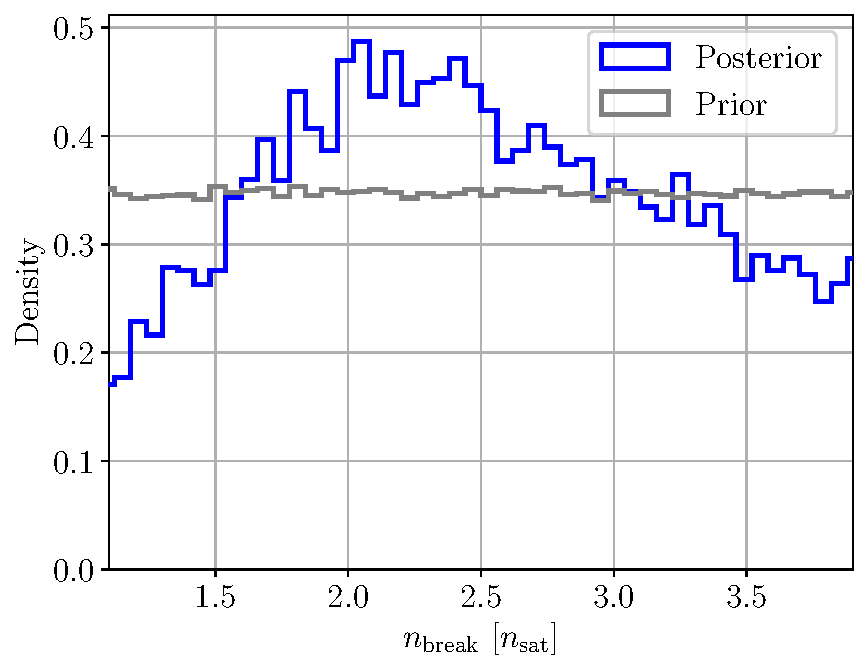
\includegraphics[width=0.55\linewidth]{Figures/nbreak_posterior.pdf}
  \end{figure}

\end{frame}

\begin{frame}{Methods -- Variational inference}

  \def\x{2mm}

  Alternative to Bayesian inference: optimization with gradients

  % \vspace{\x}

  \begin{itemize}
    \vspace{\x}

    \item $\hat{R}_i, \hat{\Lambda}_i$: ``target'' tidal deformabilities at masses $M_i$

    \vspace{\x}
    
    \item Loss function $L(\thetaeos)$: relative error in tidal deformability $\Lambda$
    
    \vspace{\x}

    \item Gradient descent: $\boldtheta^{(i+1)} \leftarrow \boldtheta^{(i)} - \gamma \nabla L(\boldtheta^{(i)})$

    \vspace{\x}

    \item Efficiently invert a complete NS family to find the EOS
  \end{itemize}

  \vspace{-3mm}

  \begin{columns}

    \column{0.5\textwidth}

    \begin{equation*}
      L(\thetaeos) = \frac1N \sum_{i=1}^N \left| \frac{\Lambda_i(\thetaeos) - \hat{\Lambda}_i}{\hat{\Lambda}_i} \right|
    \end{equation*}

    \column{0.5\textwidth}

    \begin{figure}[htpb]
      \centering
      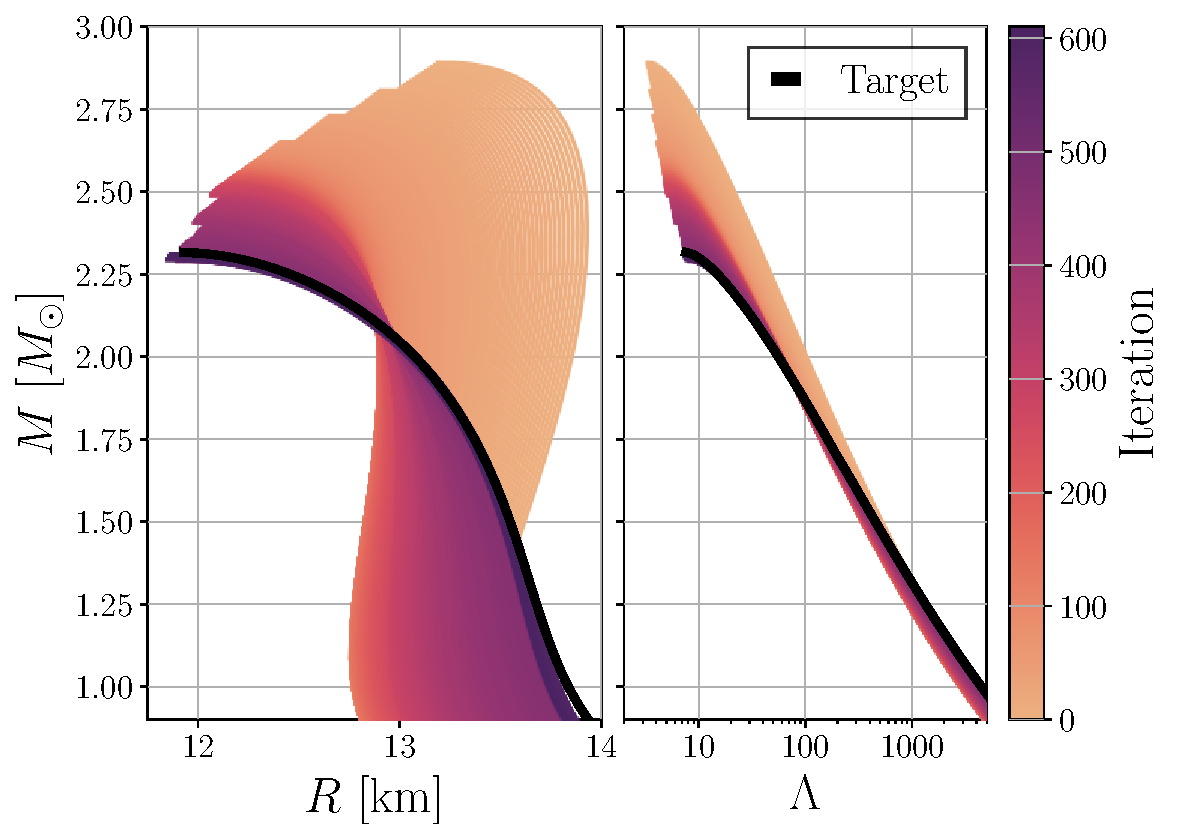
\includegraphics[width=1.0\linewidth]{Figures/showcase_variational_inference.pdf}
    \end{figure}

  \end{columns}
\end{frame}

\begin{frame}{Results -- degeneracy in metamodel parametrization}

  Only consider metamodel parameters (no $c_s^2(n)$ extension)
  
\end{frame}


\end{document}

